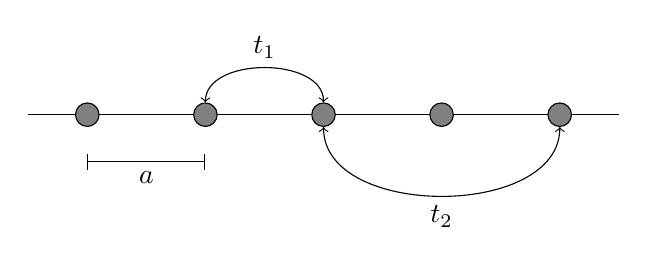
\begin{tikzpicture}[scale=1.5]
    \draw (0.5, 0) -- (5.5, 0);

    \foreach \x in {1,...,5}
    {
        \node[fill=gray, draw, circle, inner sep=3] (n\x) at (\x, 0) {};
    }

    \draw[<->, in=90, out=90] (n2) to node[midway, above] {$t_1$} (n3);
    \draw[<->, in=270, out=270] (n3) to node[midway, below] {$t_2$} (n5);

    \draw[|-|] (1, -0.4) -- ++(1, 0) node[below, midway] {$a$};
\end{tikzpicture}
